\chapter{Extensions on the evaluation results}
\label{app:Extensions on the evaluation results}

\section{Results on the testset}



\section{Old stuff}
\subsection{Removing outliers}


% some meters don't have a lot of missing values, but have very untraditional output. Two cases are looked into
% 1. big deviation from the average meter. 
% 2. a full day of zeros is included. 
% 3. the moving average changes spectaculair --> fundamental change in the energy consumption
% whitch is hard to forecast for. (not consistent with a normal consumption pattern)
% Weird meters that are identified: 2985, 2984,
% Normal meters: 2979, 2982
% idea to check also for outliers on monthly/weekly scale? 
After the missing values are replaced by estimations, the outliers of the electricity consumption signals are identified.
This is done by looking  at the z-scores of the yearly consumptions. A z-score is calculated using equation \ref{eq:z-score} and assumes that the yearly consumptions are normally distributed around the average consumption. Consumptions that have a very low probability to occur are removed by imposing that $ |z-score| < 3 $.

\begin{equation}
	z-score = \frac{x-\mu}{\sigma}
\end{equation}                      

Figure \ref{fig:z-score} gives the obtained z-values. It can be seen that $ 6 $ meters with an unlikely high or low consumption are removed. 

\begin{figure}[h!]
	\centering
	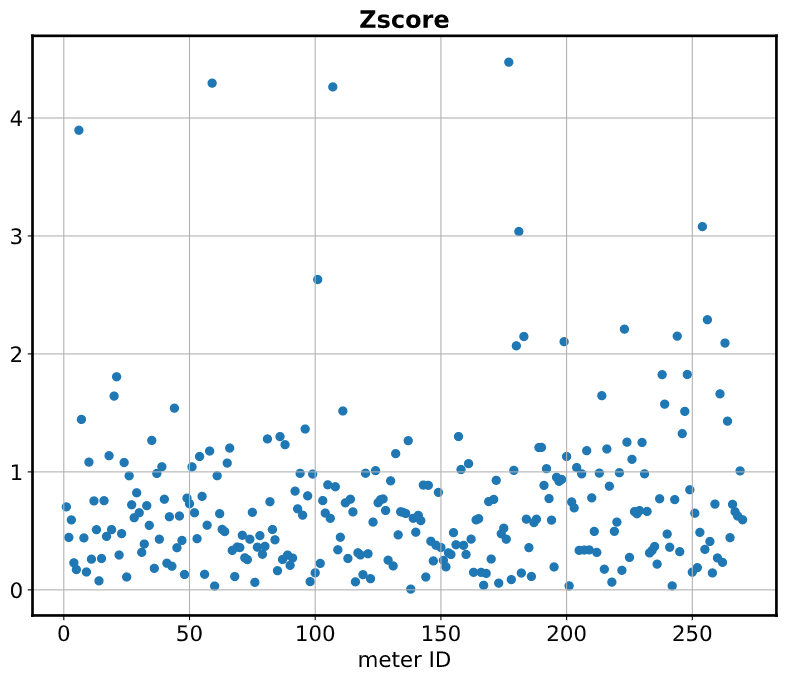
\includegraphics[width=0.8\textwidth]{z-score.png}
	\caption{Z-scores calculated from the yearly consumptions.}
	\label{fig:z-score}
\end{figure}


\subsection{Normalization of the data}
% normalize as done in ppt --> deviding by the yearly consumption.
% downside of this normalilzation that outshooters will have influence.
Normalization is necessary because while absolute consumption differs, relative patterns of human behaviour are more similar \cite{Lago2020}. The patterns in the human behaviour is what a forecasting model is trying to predict and normalization contributes by avoiding the disturbance of different magnitudes in which this human pattern may occur. Every individual household time-serie is normalized based on its maximum and minimum value according to equation \ref{eq:norm}. 

\begin{equation}\label{eq:norm}
	normalized value = \frac{x - x_{min}}{x_{max} - x_{min}}
\end{equation}  

As discussed in section \ref{s:Basic analysis} the average is taken over all the normalized time-series to obtain a single signal.\textbf{Ask if this is good??}  Because the maximum is taken into account during the normalization, measurement out shooters have an influence on the normalization. 


\section{ARIMA}
% Idea is to use the simple ARIMA model as a base line forecasting model. 
% see datacamp and youtube Lola
% ARIMA assumes stationary data.
What is ARIMA. 
Assumptions of ARIMA...

\textbf{Stationarity}\\
https://machinelearningmastery.com/remove-trends-seasonality-difference-transform-python/
When data is modelled it is assumed that the statistics of the data are consistent or stationary. This means the mean and standard deviation is not changing in time. However, because time series are often subdued to a trend or seasonality this assumption of stationarity is violated. In order to model not stationary observations by a stationary model as ARIMA, trends and seasonal effects should be removed. A way to check the stationarity of your observations, the ``Dicky-Fuller test'' can be used.
A way to remove non-stationarity is by using ``Difference Transform''. Here the trend and seasonality is subtracted from the observations leaving behind a stationary dataset.


%%% Local Variables: 
%%% mode: latex
%%% TeX-master: "thesis"
%%% End: 
